
\documentclass[letterpaper,english]{article}

%\documentclass[letterpaper,twocolumn,english]{article}
\usepackage[T1]{fontenc}
\usepackage[latin1]{inputenc}
\usepackage{graphicx}

\usepackage{geometry}
\geometry{verbose,letterpaper,tmargin=1in,bmargin=1in,lmargin=1in,rmargin=1in}

\makeatletter

\usepackage{babel}

\begin{document}

\title{LLADD Outline }


\author{Russell Sears \and ... \and Eric Brewer}

\maketitle



\begin{enumerate}

\item Abstract

\subsection*{Abstract}

% todo/rcs Need to talk about collection api stuff / generalization of ARIES / new approach to application development

Although many systems provide transactionally consistent data
management, existing implementations are generally monolithic and tied
to a higher-level DBMS, limiting the scope of their usefulness to a
single application or a specific type of problem. As a result, many
systems are forced to ``work around'' the data models provided by a
transactional storage layer. Manifestations of this problem include
``impedance mismatch'' in the database world and the limited number of
data models provided by existing libraries such as Berkeley DB. In
this paper, we describe a light-weight, easily extensible library,
LLADD, that allows application developers to develop scalable and
transactional application-specific data structures. We demonstrate
that LLADD is simpler than prior systems, is very flexible and
performs favorably in a number of micro-benchmarks. We also describe,
in simple and concrete terms, the issues inherent in the design and
implementation of robust, scalable transactional data structures. In
addition to the source code, we have also made a comprehensive suite
of unit-tests, API documentation, and debugging mechanisms publicly
available.%
\footnote{http://lladd.sourceforge.net/%
}

\item Introduction 

\begin{enumerate}

% rcs: The original intro is left intact in the other file; it would be too hard to merge right now.

  % This paragraph is a too narrow; the original was too vague 
  \item {\bf Current transactional systems handle conventional workloads
  well, but object persistence mechanisms are a mess, as are
  {}``version oriented'' data stores requiring large, efficient atomic
  updates.}

  \item {\bf {}``Impedance mismatch'' is a term that refers to a mismatch
  between the data model provided by the data store and the data model
  required by the application. A significant percentage of software
  development effort is related to dealing with this problem. Related
  problems that have had less treatment in the literature involve
  mismatches between other performance-critical and labor intensive
  programming primitives such as concurrency models, error handling
  techniques and application development patterns.}
% rcs: see ##1## in other file for more examples
  \item {\bf Past trends in the Database community have been driven by
  demand for tools that allow extremely specialized (but commercially
  important!)  types of software to be developed quickly and
  inexpensively. {[}System R, OODBMS, benchmarks, streaming databases,
  etc{]} This has led to the development of large, monolithic database
  severs that perform well under many circumstances, but that are not
  nearly as flexible as modern programming languages or typical
  in-memory data structure libraries {[}Java Collections,
  STL{]}. Historically, programming language and software library
  development has focused upon the production of wide array of
  composable general purpose tools, allowing the application developer
  to pick algorithms and data structures that are most appropriate for
  the problem at hand.}

  \item {\bf In the past, modular database and transactional storage
  implementations have hidden the complexities of page layout,
  synchronization, locking, and data structure design under relatively
  narrow interfaces, since transactional storage algorithms'
  interdependencies and requirements are notoriously complicated.}

  \item {\bf With these trends in mind, we have implemented a modular
  version of ARIES that makes as few assumptions as possible about
  application data structures or workload. Where such assumptions are
  inevitable, we have produced narrow APIs that allow the application
  developer to plug in alternative implementations of the modules that
  comprise our ARIES implementation. Rather than hiding the underlying
  complexity of the library from developers, we have produced narrow,
  simple API's and a set of invariants that must be maintained in
  order to ensure transactional consistency, allowing application
  developers to produce high-performance extensions with only a little
  effort.}

\end{enumerate}
\item {\bf 2.Prior work}

\begin{enumerate}

  \item{\bf Databases' Relational model leads to performance /
  representation problems.}

On the database side of things, relational databases excel in areas
where performance is important, but where the consistency and
durability of the data are crucial.  Often, databases significantly
outlive the software that uses them, and must be able to cope with
changes in business practices, system architectures,
etc.~\cite{relational}

Databases are designed for circumstances where development time may
dominate cost, many users must share access to the same data, and
where security, scalability, and a host of other concerns are
important.  In many, if not most circumstances these issues are less
important, or even irrelevant.  Therefore, applying a database in
these situations is likely overkill, which may partially explain the
popularity of MySQL~\cite{mysql}, which allows some of these
constraints to be relaxed at the discretion of a developer or end
user.

  \item{\bf OODBMS / XML database systems provide model tied closely to PL
  or hierarchical formats, but, like the relational model, these
  models are extremely general, and might be inappropriate for
  applications with stringent performance demands, or that use these
  models in a way that cannot be supported well with the database
  system's underlying data structures.}

Object-oriented databases are more focused on facilitating the
development of complex applications that require reliable storage and
may take advantage of less-flexible, more efficient data models, as
they often only interact with a single application, or a handful of
variants of that application.~\cite{lamb}

  \item{\bf Berkeley DB provides a lower level interface, increasing
  performance, and providing efficient tree and hash based data
  structures, but hides the details of storage management and the
  primitives provided by its transactional layer from
  developers. Again, only a handful of data formats are made available
  to the developer.}

%rcs: The inflexibility of databases has not gone unnoticed ... or something like that.

Still, there are many applications where MySQL is too inflexible.  In
order to serve these applications, a host of software solutions have
been devised.  Some are extremely complex, such as semantic file
systems, where the file system understands the contents of the files
that it contains, and is able to provide services such as rapid
search, or file-type specific operations such as thumb-nailing,
automatic content updates, and so on.  Others are simpler, such as
Berkeley~DB,~\cite{berkeleyDB, bdb} which provides transactional
storage of data in unindexed form, or in indexed form using a hash
table or tree.  LRVM is a version of malloc() that provides
transactional memory, and is similar to an object-oriented database
but is much lighter weight, and more flexible~\cite{lrvm}.

  \item {\bf Incredibly scalable, simple servers CHT's, google fs?, ...}

Finally, some applications require incredibly simple, but extremely
scalable storage mechanisms.  Cluster hash tables are a good example
of the type of system that serves these applications well, due to
their relative simplicity, and extremely good scalability
characteristics.  Depending on the fault model on which a cluster hash
table is implemented, it is quite plausible that key portions of the
transactional mechanism, such as forcing log entries to disk, will be
replaced with other durability schemes, such as in-memory replication
across many nodes, or multiplexing log entries across multiple
systems.  This level of flexibility would be difficult to retrofit
into existing transactional applications, but is often important in
the environments in which these applications are deployed.


  \item {\bf Implementations of ARIES and other transactional storage
  mechanisms include many of the useful primitives described below,
  but prior implementations either deny application developers access
  to these primitives {[}??{]}, or make many high-level assumptions
  about data representation and workload {[}DB Toolkit from
  Wisconsin??-need to make sure this statement is true!{]}}

\end{enumerate}

\item {\bf 3.Architecture  }

  % rcs:The last paper contained a tutorial on how to use LLADD, which 
  % should be shortend or removed from this version, so I didn't paste it 
  % in.  However, it made some points that belong in this section
  % see: ##2##

\begin{enumerate}
  %
  % need block diagram here.  4 blocks:
  %
  % App specific:
  %
  %  - operation wrapper
  %  - operation redo fcn
  %
  % LLADD core:
  % 
  %  - logger
  %  - page file
  %
  % lock manager, etc can come later...
  %

  \item {\bf {}``Core LLADD'' vs {}``Operations''}

A LLADD operation consists of some code that manipulates data that has
been stored in transactional pages.  These operations implement
high-level actions that are composed into transactions.  They are
implemented at a relatively low level, and have full access to the
ARIES algorithm.  Applications are implemented on top of the
interfaces provided by an application-specific set of operations.
This allows the the application, the operation, and LLADD itself to be
independently improved.  We have implemented a number of extremely
simple, high performance general purpose data structures for our
sample applications, and as building blocks for new data structures.
Example data structures include two distinct linked list
implementations, and an extendible array.  Surprisingly, even these
simple operations have important performance characteristics that are
not provided by existing systems.

  \item {\bf  ARIES provides {}``transactional pages'' }

\begin{enumerate}

  \item {\bf Diversion on ARIES semantics }
  
    %rcs: Is this the best way to describe this?

  \item {\bf Non-interleaved transactions vs. Nested top actions
  vs. Well-ordered writes.}

    % key point: locking + nested top action = 'normal' multithreaded
    %software development! (modulo 'obvious' mistakes like algorithmic
    %errors in data structures, errors in the log format, etc)
    
    % second point: more difficult techniques can be used to optimize
    % log bandwidth. _in ways that other techniques cannot provide 
    % to application developers.

Instead of providing a comprehensive discussion of ARIES, we will
focus upon those features of the algorithm that are most relevant
to a developer attempting to add a new set of operations. Correctly
implementing such extensions is complicated by concerns regarding
concurrency, recovery, and the possibility that any operation may
be rolled back at runtime.

We first sketch the constraints placed upon operation implementations,
and then describe the properties of our implementation that
make these constraints necessary. Because comprehensive discussions of
write ahead logging protocols and ARIES are available elsewhere,~\cite{haerder, aries} we
only discuss those details relevant to the implementation of new
operations in LLADD.


\subsection{Properties of an Operation\label{sub:OperationProperties}}


Since transactions may be aborted,
the effects of an operation must be reversible. Furthermore, aborting
and committing transactions may be interleaved, and LLADD does not
allow cascading aborts,%
\footnote{That is, by aborting, one transaction may not cause other transactions
to abort. To understand why operation implementors must worry about
this, imagine that transaction A split a node in a tree, transaction
B added some data to the node that A just created, and then A aborted.
When A was undone, what would become of the data that B inserted?%
} so in order to implement an operation, we must implement some sort
of locking, or other concurrency mechanism that isolates transactions
from each other. LLADD only provides physical consistency; due to the variety of locking systems available, and their interaction with application workload,~\cite{multipleGenericLocking} we leave
it to the application to decide what sort of transaction isolation is
appropriate.  

For example, it is relatively easy to
build a strict two-phase locking lock manager~\cite{hierarcicalLocking} on top of LLADD, as
needed by a DBMS, or a simpler lock-per-folder approach that would
suffice for an IMAP server.  Thus, data dependencies among
transactions are allowed, but we still must ensure the physical
consistency of our data structures, such as operations on pages or locks.

Also, all actions performed by a transaction that committed must be
restored in the case of a crash, and all actions performed by aborting
transactions must be undone. In order for LLADD to arrange for this
to happen at recovery, operations must produce log entries that contain
all information necessary for undo and redo.

An important concept in ARIES is the ``log sequence number'' or LSN.
An LSN is essentially a virtual timestamp that goes on every page; it
marks  the last log entry that is reflected on the page, and
implies that all previous log entries are also reflected. Given the
LSN, LLADD calculates where to start playing back the log to bring the page
up to date.  The LSN goes on the page so that it is always written to
disk atomically with the data on the page.

ARIES (and thus LLADD) allows pages to be {\em stolen}, i.e. written
back to disk while they still contain uncommitted data.  It is
tempting to disallow this, but to do so has serious consequences such as
a increased need for buffer memory (to hold all dirty pages). Worse,
as we allow multiple transactions to run concurrently on the same page
(but not typically the same item), it may be that a given page {\em
always} contains some uncommitted data and thus could never be written
back to disk.  To handle stolen pages, we log UNDO records that
we can use to undo the uncommitted changes in case we crash.  LLADD
ensures that the UNDO record is durable in the log before the
page is written back to disk and that the page LSN reflects this log entry.

Similarly, we do not force pages out to disk every time a transaction
commits, as this limits performance.  Instead, we log REDO records
that we can use to redo the change in case the committed version never
makes it to disk.  LLADD ensures that the REDO entry is durable in the
log before the transaction commits.  REDO entries are physical changes
to a single page (``page-oriented redo''), and thus must be redone in
the exact order.

One unique aspect of LLADD, which
is not true for ARIES, is that {\em normal} operations use the REDO
function; i.e. there is no way to modify the page except via the REDO
operation.  This has the great property that the REDO code is known to
work, since even the original update is a ``redo''.
In general, the LLADD philosophy is that you
define operations in terms of their REDO/UNDO behavior, and then build
the actual update methods around those.

Eventually, the page makes it to disk, but the REDO entry is still
useful: we can use it to roll forward a single page from an archived
copy.  Thus one of the nice properties of LLADD, which has been
tested, is that we can handle media failures very gracefully: lost
disk blocks or even whole files can be recovered given an old version
and the log.  

\subsection{Normal Processing}

Operation implementors follow the pattern in Figure \ref{cap:Tset},
and need only implement a wrapper function (``Tset()'' in the figure,
and register a pair of redo and undo functions with LLADD.
The Tupdate function, which is built into LLADD, handles most of the
runtime complexity.  LLADD uses the undo and redo functions
during recovery in the same way that they are used during normal
processing.  

The complexity of the ARIES algorithm lies in determining
exactly when the undo and redo operations should be applied.  LLADD 
handles these details for the implementors of operations.


\subsubsection{The buffer manager}

LLADD manages memory on behalf of the application and prevents pages
from being stolen prematurely. Although LLADD uses the STEAL policy
and may write buffer pages to disk before transaction commit, it still
must make sure that the UNDO log entries have been forced to disk
before the page is written to disk. Therefore, operations must inform
the buffer manager when they write to a page, and update the LSN of
the page. This is handled automatically by the write methods that LLADD 
provides to operation implementors (such as writeRecord()). However,
it is also possible to create your own low-level page manipulation
routines, in which case these routines must follow the protocol.


\subsubsection{Log entries and forward operation\\ (the Tupdate() function)\label{sub:Tupdate}}

In order to handle crashes correctly, and in order to undo the
effects of aborted transactions, LLADD provides operation implementors
with a mechanism to log undo and redo information for their actions.
This takes the form of the log entry interface, which works as follows.
Operations consist of a wrapper function that performs some pre-calculations
and perhaps acquires latches. The wrapper function then passes a log
entry to LLADD. LLADD passes this entry to the logger, {\em and then processes
it as though it were redoing the action during recovery}, calling a function
that the operation implementor registered with
LLADD. When the function returns, control is passed back to the wrapper
function, which performs any post processing (such as generating return
values), and releases any latches that it acquired. %
\begin{figure}
%\begin{center}
%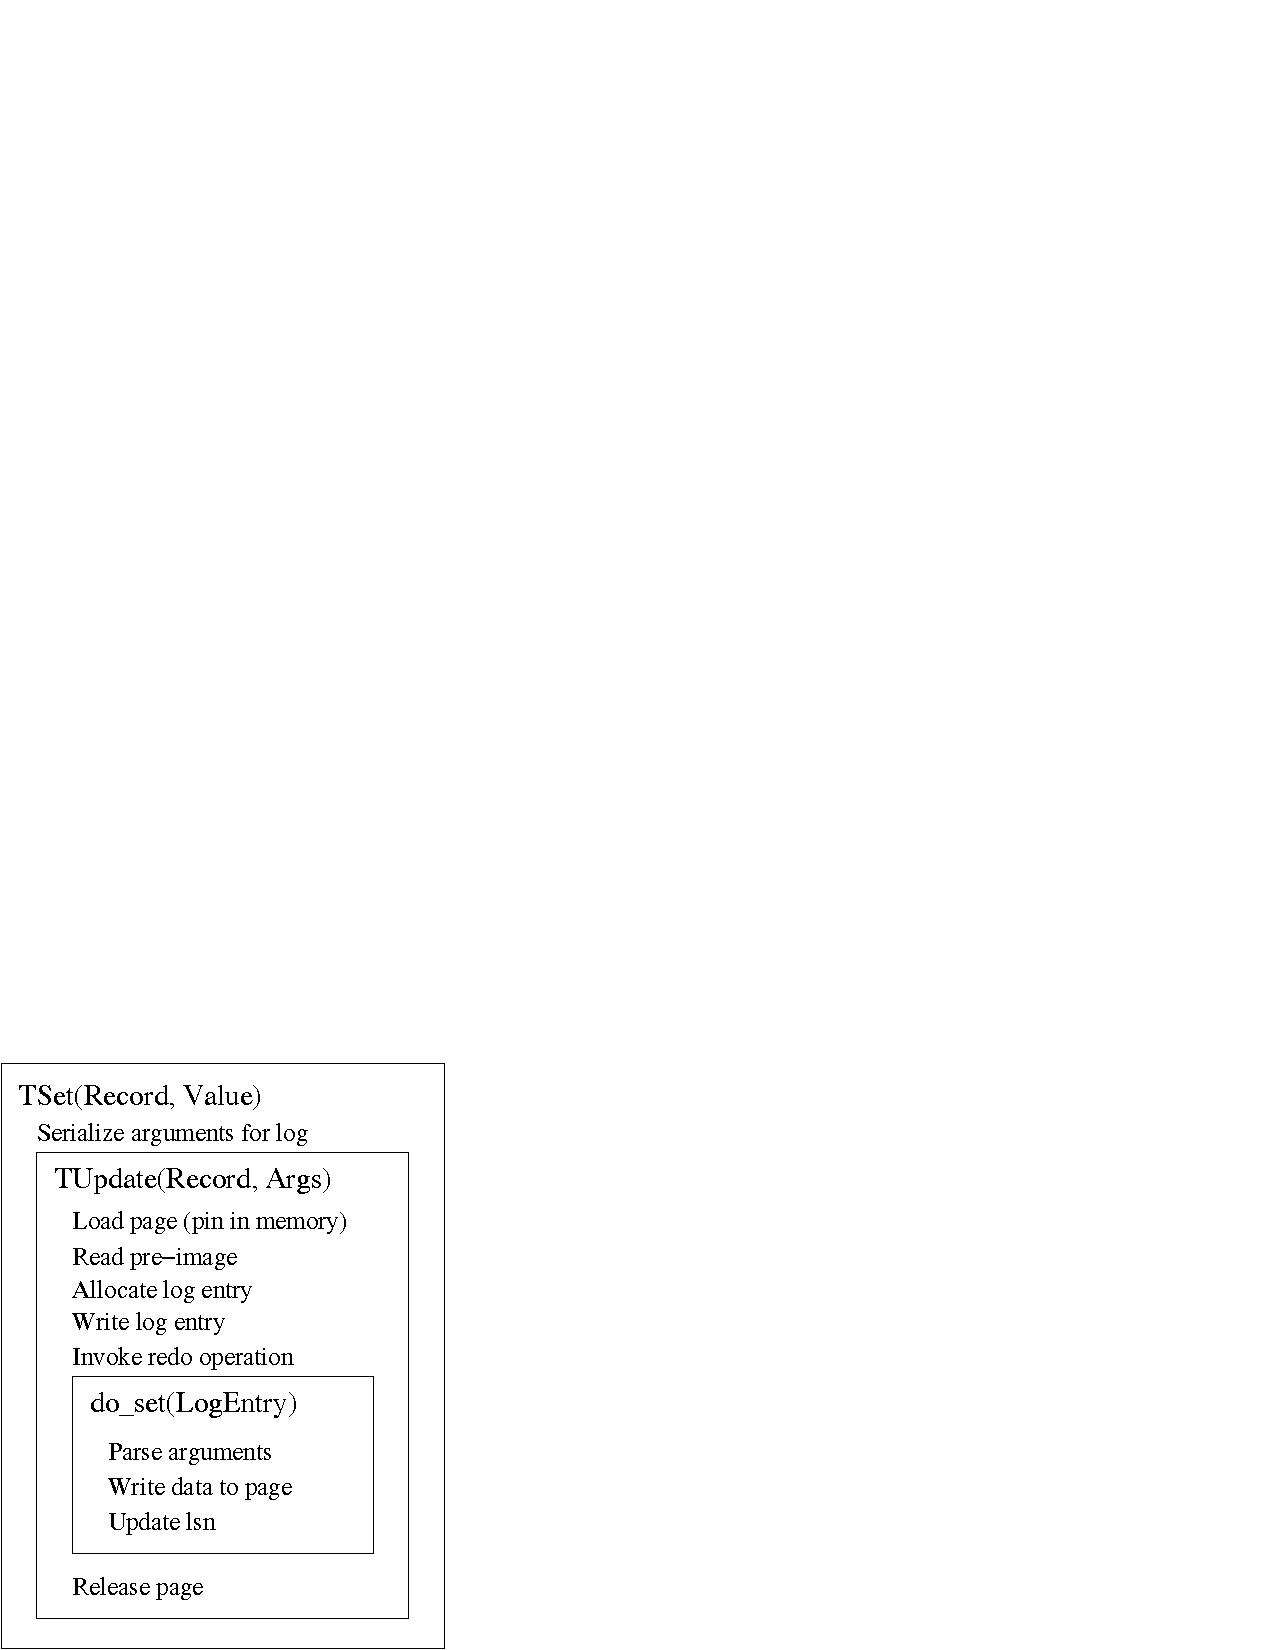
\includegraphics[%
%  width=0.70\columnwidth]{TSetCall.pdf}
%\end{center}

\caption{\label{cap:Tset}Runtime behavior of a simple operation. Tset() and redoSet() are
extensions that implement a new operation, while Tupdate() is built in. New operations
need not be aware of the complexities of LLADD.}
\end{figure}


This way, the operation's behavior during recovery's redo phase (an
uncommon case) will be identical to the behavior during normal processing,
making it easier to spot bugs. Similarly, undo and redo operations take
an identical set of parameters, and undo during recovery is the same 
as undo during normal processing.  This makes recovery bugs more obvious and allows redo
functions to be reused to implement undo. 

Although any latches acquired by the wrapper function will not be
reacquired during recovery, the redo phase of the recovery process
is single threaded. Since latches acquired by the wrapper function
are held while the log entry and page are updated, the ordering of
the log entries and page updates associated with a particular latch
will be consistent. Because undo occurs during normal operation, 
some care must be taken to ensure that undo operations obtain the 
proper latches.


\subsection{Recovery}

In this section, we present the details of crash recovery, user-defined logging, and atomic actions that commit even if their enclosing transaction aborts.

\subsubsection{ANALYSIS / REDO / UNDO}

Recovery in ARIES consists of three stages, analysis, redo and undo. 
The first, analysis, is
implemented by LLADD, but will not be discussed in this
paper. The second, redo, ensures that each redo entry in the log 
will have been applied to each page in the page file exactly once.
The third phase, undo, rolls back any transactions that were active
when the crash occurred, as though the application manually aborted
them with the {}``abort'' function call.
  
After the analysis phase, the on-disk version of the page file
is in the same state it was in when LLADD crashed. This means that
some subset of the page updates performed during normal operation
have made it to disk, and that the log contains full redo and undo
information for the version of each page present in the page file.%
\footnote{Although this discussion assumes that the entire log is present, the
ARIES algorithm supports log truncation, which allows us to discard
old portions of the log, bounding its size on disk.%
} Because we make no further assumptions regarding the order in which
pages were propagated to disk, redo must assume that any
data structures, lookup tables, etc. that span more than a single
page are in an inconsistent state. Therefore, as the redo phase re-applies
 the information in the log to the page file, it must address all pages directly. 

This implies that the redo information for each operation in the log
must contain the physical address (page number) of the information
that it modifies, and the portion of the operation executed by a single
redo log entry must only rely upon the contents of the page that the 
entry refers to. Since we assume that pages are propagated to disk
atomically, the REDO phase may rely upon information contained within
a single page.

Once redo completes, we have applied some prefix of the run-time log.
Therefore, we know that the page file is in
a physically consistent state, although it contains portions of the
results of uncommitted transactions. The final stage of recovery is
the undo phase, which simply aborts all uncommitted transactions. Since
the page file is physically consistent, the transactions may be aborted
exactly as they would be during normal operation. 


\subsubsection{Physical, Logical and Phisiological Logging.}

The above discussion avoided the use of some common terminology 
that should be presented here. {\em Physical logging } 
is the practice of logging physical (byte-level) updates
and the physical (page number) addresses to which they are applied.

{\em Physiological logging } is what LLADD recommends for its redo 
records. The physical address (page number) is stored, but the byte offset
and the actual difference are stored implicitly in the parameters
of the redo or undo function. These parameters allow the function to 
update the page in a way that preserves application semantics.
One common use for this is {\em slotted pages}, which use an on-page level of 
indirection to allow records to be rearranged within the page; instead of using the page offset, redo 
operations use a logical offset to locate the data. This allows data within
a single page to be re-arranged at runtime to produce contiguous
regions of free space. LLADD generalizes this model; for example, the parameters passed to the function may utilize application specific properties in order to be significantly smaller than the physical change made to the page.~\cite{physiological}

{\em Logical logging } can only be used for undo entries in LLADD,
and is identical to physiological logging, except that it stores a
logical address (the key of a hash table, for instance) instead of
a physical address. This allows the location of data in the page file
to change, even if outstanding transactions may have to roll back
changes made to that data. Clearly, for LLADD to be able to apply
logical log entries, the page file must be physically consistent,
ruling out use of logical logging for redo operations.

LLADD supports all three types of logging, and allows developers to
register new operations, which is the key to its extensibility. After
discussing LLADD's architecture, we will revisit this topic with a
concrete example.


\subsection{Concurrency and Aborted Transactions}

Section~\ref{sub:OperationProperties} states that LLADD does not
allow cascading aborts, implying that operation implementors must
protect transactions from any structural changes made to data structures
by uncommitted transactions, but LLADD does not provide any mechanisms
designed for long-term locking. However, one of LLADD's goals is to
make it easy to implement custom data structures for use within safe,
multi-threaded transactions. Clearly, an additional mechanism is needed.

The solution is to allow portions of an operation to ``commit'' before
the operation returns.\footnote{We considered the use of nested top actions, which LLADD could easily
support. However, we currently use the slightly simpler (and lighter-weight)
mechanism described here. If the need arises, we will add support
for nested top actions.}
An operation's wrapper is just a normal function, and therefore may
generate multiple log entries. First, it writes an undo-only entry
to the log. This entry will cause the \emph{logical} inverse of the
current operation to be performed at recovery or abort, must be idempotent,
and must fail gracefully if applied to a version of the database that
does not contain the results of the current operation. Also, it must
behave correctly even if an arbitrary number of intervening operations
are performed on the data structure.

Next, the operation writes one or more redo-only log entries that may perform structural
modifications to the data structure. These redo entries have the constraint that any prefix of them must leave the database in a consistent state, since only a prefix might execute before a crash.  This is not as hard as it sounds, and in fact the
$B^{LINK}$ tree~\cite{blink} is an example of a B-Tree implementation
that behaves in this way, while the linear hash table implementation
discussed in Section~\ref{sub:Linear-Hash-Table} is a scalable 
hash table that meets these constraints.

%[EAB: I still think there must be a way to log all of the redoes
%before any of the actions take place, thus ensuring that you can redo
%the whole thing if needed. Alternatively, we could pin a page until
%the set completes, in which case we know that that all of the records
%are in the log before any page is stolen.]

\subsection{Summary}

This section presented a relatively simple set of rules and patterns
that a developer must follow in order to implement a durable, transactional
and highly-concurrent data structure using LLADD:

\begin{itemize}
\item Pages should only be updated inside of a redo or undo function.
\item An update to a page should update the LSN. 
\item If the data read by the wrapper function must match the state of
the page that the redo function sees, then the wrapper should latch
the relevant data.
\item Redo operations should address pages by their physical offset,
while Undo operations should use a more permanent address (such as
index key) if the data may move between pages over time.
\item An undo operation must correctly update a data structure if any
prefix of its corresponding redo operations are applied to the
structure, and if any number of intervening operations are applied to
the structure.
\end{itemize}
Because undo and redo operations during normal operation and recovery
are similar, most bugs will be found with conventional testing
strategies.  It is difficult to verify the final property, although a
number of tools could be written to simulate various crash scenarios,
and check the behavior of operations under these scenarios.  Of course, 
such a tool could easily be applied to existing LLADD operations.

Note that the ARIES algorithm is extremely complex, and we have left
out most of the details needed to understand how ARIES works, or to 
implement it correctly.
Yet, we believe we have covered everything that a programmer needs
 to know in order to implement new data structures using the 
functionality that ARIES provides. This was possible due to the encapsulation
of the ARIES algorithm inside of LLADD, which is the feature that
most strongly differentiates LLADD from other, similar libraries.
We hope that this will increase the availability of transactional
data primitives to application developers.



\end{enumerate}

  \item {\bf Log entries as a programming primitive }

  %rcs: Not quite happy with existing text; leaving this section out for now.
  %
  %  Need to make some points the old text did not make:
  %
  %     - log optimizations (for space) can be very important.  
  %           - many small writes 
  %           - large write of small diff 
  %           - app overwrites page many times per transaction (for example, database primary key)
  %    We have solutions to #1 and 2.  A general solution to #3 involves 'scrubbing' a logical log of redundant operations.
  %    
  %        - Talk about virtual async log thing...

  \item {\bf Error handling with compensations as {}``abort() for C''}

  % stylized usage of Weimer -> cheap error handling, no C compiler modifications...

  \item {\bf Concurrency models are fundamentally application specific, but
  record/page level locking and index locks are often a nice trade-off}

  \item {\bf {}``latching'' vs {}``locking'' - data structures internal to
  LLADD are protected by LLADD, allowing applications to reason in
  terms of logical data addresses, not physical representation. Since
  the application may define a custom representation, this seems to be
  a reasonable tradeoff between application complexity and
  performance.}

\end{enumerate}

\item {\bf Applications }

\begin{enumerate}

  \item {\bf Atomic file-based transactions. Prototype blob implementation
  using force, shadow copies (trivial to implement given transactional
  pages).  File systems that implement atomic operations may allow
  data to be stored durably without calling flush() on the data
  file. Current implementation useful for blobs that are typically
  changed entirely from update to update, but smarter implementations
  are certainly possible. The blob implementation primarily consists
  of special log operations that cause file system calls to be made at
  appropriate times, and is simple, so it could easily be replaced by
  an application that frequently update small ranges within blobs, for
  example.}

  \item {\bf Index implementation - modular hash table. Relies on separate
  linked list, expandable array implementations.}

\subsection{Array List}
   % Example of how to avoid nested top actions
\subsection{Linked Lists}
   % Example of two different page allocation strategies.
   % Explain how to implement linked lists w/out NTA's (even though we didn't do that)?

\subsection{Linear Hash Table\label{sub:Linear-Hash-Table}}
   % The implementation has changed too much to directly reuse old section, other than description of linear hash tables:

Linear hash tables are hash tables that are able to extend their bucket
list incrementally at runtime. They work as follows. Imagine that
we want to double the size of a hash table of size $2^{n}$, and that
the hash table has been constructed with some hash function $h_{n}(x)=h(x)\, mod\,2^{n}$.
Choose $h_{n+1}(x)=h(x)\, mod\,2^{n+1}$ as the hash function for
the new table. Conceptually we are simply prepending a random bit
to the old value of the hash function, so all lower order bits remain
the same. At this point, we could simply block all concurrent access
and iterate over the entire hash table, reinserting values according
to the new hash function. 

However, because of the way we chose $h_{n+1}(x),$ we know that the
contents of each bucket, $m$, will be split between bucket $m$ and
bucket $m+2^{n}$. Therefore, if we keep track of the last bucket
that was split, we can split a few buckets at a time, resizing the
hash table without introducing long pauses while we reorganize the
hash table~\cite{lht}. We can handle overflow using standard techniques;
LLADD's linear hash table uses linked lists of overflow buckets.

% Implementation simple!  Just slap together the stuff from the prior two sections, and add a header + bucket locking.

  \item {\bf Asynchronous log implementation/Fast writes. Prioritization of
  log writes (one {}``log'' per page) implies worst case performance
  (write, then immediate read) will behave on par with normal
  implementation, but writes to portions of the database that are not
  actively read should only increase system load (and not directly
  increase latency)}

  \item {\bf Custom locking. Hash table can support all of the SQL degrees
  of transactional consistency, but can also make use of
  application-specific invariants and synchronization to accommodate
  deadlock-avoidance, which is the model most naturally supported by C
  and other programming languages.}

%Many plausible lock managers, can do any one you want.
%too much implemented part of DB; need more 'flexible' substrate.

\end{enumerate}

\item {\bf Validation }

\begin{enumerate}

  \item {\bf Serialization Benchmarks (Abstract log) }

    % Need to define application semantics workload (write heavy w/ periodic checkpoint?) that allows for optimization.
    
    % All of these graphs need X axis dimensions.  Number of (read/write?) threads, maybe?
 
    % Graph 1:  Peak write throughput. Abstract log runs everything else into the ground (no disk i/o, basically, measure
    % contention on ringbuffer...)

    % Graph 2:  Measure maximum average write throughput: Write throughput vs. rate of log growth.  Spool abstract log to disk.
    %           Reads starve, or read stale data.

    % Graph 3:  Latency @ peak steady state write throughput.  Abstract log size remains constant.  Measure read latency vs.
    %           queue length.

  \item {\bf Graph traversal benchmarks:  Bulk load + hot and cold transitive closure queries}

  \item {\bf Hierarchical Locking - Proof of concept}

  \item {\bf TPC-C (Flexibility) - Proof of concept}
    
   % Abstract syntax tree implementation?

  \item {\bf Sample Application. (Don't know what yet?) }

\end{enumerate}

\item {\bf Future work}
  \item {\bf PL / Testing stuff}
  \item {\bf Explore async log capabilities further}

\item {\bf Conclusion}

\end{enumerate}

\begin{thebibliography}{99}

\bibitem[1]{multipleGenericLocking} Agrawal, et al. {\em Concurrency Control Performance Modeling: Alternatives and Implications}. TODS 12(4): (1987) 609-654

\bibitem[2]{bdb} Berkeley~DB, {\tt http://www.sleepycat.com/}

\bibitem[3]{capriccio} R. von Behren, J Condit, F. Zhou, G. Necula, and E. Brewer. {\em Capriccio: Scalable Threads for Internet Services} SOSP 19 (2003).

\bibitem[4]{relational} E. F. Codd, {\em A Relational Model of Data for Large Shared Data Banks.} CACM 13(6) p. 377-387 (1970)

\bibitem[5]{lru2s} Envangelos P. Markatos. {\em On Caching Search Engine Results}.  Institute of Computer Science, Foundation for Research \& Technology - Hellas (FORTH) Technical Report 241 (1999)

\bibitem[6]{semantic} David K. Gifford, P. Jouvelot, Mark A. Sheldon, and Jr. James W. O'Toole. {\em Semantic file systems}. Proceedings of the Thirteenth ACM Symposium on Operating Systems Principles, (1991) p. 16-25.

\bibitem[7]{physiological} Gray, J. and Reuter, A. {\em Transaction Processing: Concepts and Techniques}. Morgan Kaufmann (1993) San Mateo, CA

\bibitem[8]{hierarcicalLocking} Jim Gray, Raymond A. Lorie, and Gianfranco R. Putzulo. {\em Granularity of locks and degrees of consistency in a shared database}. In 1st International Conference on VLDB, pages 428--431, September 1975. Reprinted in Readings in Database Systems, 3rd edition.

\bibitem[9]{haerder} Haerder \& Reuter {\em "Principles of Transaction-Oriented Database Recovery." } Computing Surveys 15(4) p 287-317 (1983)

\bibitem[10]{lamb} Lamb, et al., {\em The ObjectStore System.} CACM 34(10) (1991) p. 50-63

\bibitem[11]{blink} Lehman \& Yao, {\em Efficient Locking for Concurrent Operations in B-trees.} TODS 6(4) (1981) p. 650-670

\bibitem[12]{lht} Litwin, W., {\em Linear Hashing: A New Tool for File and Table Addressing}. Proc. 6th VLDB, Montreal, Canada, (Oct. 1980) p. 212-223

\bibitem[13]{aries} Mohan, et al., {\em ARIES: A Transaction Recovery Method Supporting Fine-Granularity Locking and Partial Rollbacks Using Write-Ahead Logging.} TODS 17(1) (1992) p. 94-162

\bibitem[14]{twopc} Mohan, Lindsay \& Obermarck, {\em Transaction Management in the R* Distributed Database Management System} TODS 11(4) (1986) p. 378-396

\bibitem[15]{ariesim} Mohan, Levine. {\em ARIES/IM: an efficient and high concurrency index management method using write-ahead logging} International Converence on Management of Data, SIGMOD (1992) p. 371-380

\bibitem[16]{mysql} {\em MySQL}, {\tt http://www.mysql.com/ }

\bibitem[17]{reiser} Reiser,~Hans~T. {\em ReiserFS 4} {\tt http://www.namesys.com/ } (2004)
%
\bibitem[18]{berkeleyDB} M. Seltzer, M. Olsen. {\em LIBTP: Portable, Modular Transactions for UNIX}. Proceedings of the 1992 Winter Usenix (1992)

\bibitem[19]{lrvm} Satyanarayanan, M., Mashburn, H. H., Kumar, P., Steere, D. C., AND Kistler, J. J. {\em Lightweight Recoverable Virtual Memory}. ACM Transactions on Computer Systems 12, 1 (Februrary 1994) p. 33-57. Corrigendum: May 1994, Vol. 12, No. 2, pp. 165-172.

\bibitem[20]{newTypes} Stonebraker. {\em Inclusion of New Types in Relational Data Base } ICDE (1986) p. 262-269

%\bibitem[SLOCCount]{sloccount} SLOCCount, {\tt http://www.dwheeler.com/sloccount/ }
%
%\bibitem[lcov]{lcov} The~LTP~gcov~extension, {\tt http://ltp.sourceforge.net/coverage/lcov.php }
%


%\bibitem[Beazley]{beazley} D.~M.~Beazley and P.~S.~Lomdahl, 
%{\em Message-Passing Multi-Cell Molecular Dynamics on the Connection
%Machine 5}, Parall.~Comp.~ 20 (1994) p. 173-195.
%
%\bibitem[RealName]{CitePetName} A.~N.~Author and A.~N.~Other, 
%{\em Title of Riveting Article}, JournalName VolNum (Year) p. Start-End
%
%\bibitem[ET]{embed} Embedded Tk, \\
%{\tt ftp://ftp.vnet.net/pub/users/drh/ET.html}
%
%\bibitem[Expect]{expect} Don Libes, {\em Exploring Expect}, O'Reilly \& Associates, Inc. (1995).
%
%\bibitem[Heidrich]{heidrich} Wolfgang Heidrich and Philipp Slusallek, {\em
%Automatic Generation of Tcl Bindings for C and C++ Libraries.},
%USENIX 3rd Annual Tcl/Tk Workshop (1995).
%
%\bibitem[Ousterhout]{ousterhout} John K. Ousterhout, {\em Tcl and the Tk Toolkit}, Addison-Wesley Publishers (1994).
%
%\bibitem[Perl5]{perl5} Perl5 Programmers reference,\\
%{\tt http://www.metronet.com/perlinfo/doc}, (1996).
%
%\bibitem[Wetherall]{otcl} D. Wetherall, C. J. Lindblad, ``Extending Tcl for
%Dynamic Object-Oriented Programming'', Proceedings of the USENIX 3rd Annual Tcl/Tk Workshop (1995).

\end{thebibliography}



\end{document}
